\documentclass{article}
\usepackage{amsfonts}
\usepackage{graphicx}
\usepackage[margin=1in]{geometry}
\usepackage{bm}
\usepackage{amsmath}
\usepackage{authblk}

\title{Taxonomic Enrichment Analysis with Isometric Log-Ratios}
\author[1,2]{Quang P. Nguyen}
\author[1,2]{Anne G. Hoen}
\author[1]{H. Robert Frost}
\affil[1]{Department of Biomedical Data Science, Geisel School of Medicine at Dartmouth College, Hanover, NH 03755, USA}
\affil[2]{Department of Epidemiology, Geisel School of Medicine at Dartmouth College, Hanover, NH 03755, USA}
\date{}                     %% if you don't need date to appear
\setcounter{Maxaffil}{0}
\renewcommand\Affilfont{\itshape\small}

\begin{document}
\maketitle

\begin{abstract}
    Lorem ipsum dolor sit amet, consectetur adipiscing elit. Pellentesque arcu libero, suscipit sed enim nec, posuere eleifend nunc. Phasellus vitae augue orci. Sed vestibulum nisi id augue porta, a sagittis magna accumsan. Sed augue mi, venenatis sed fringilla nec, ultrices id ipsum. Suspendisse ac sapien eu mi laoreet fringilla. Nulla facilisi. Sed eget feugiat erat, et efficitur risus. Duis sit amet nulla at leo dignissim porta. Morbi nec ligula non sapien fringilla congue. Proin consequat volutpat nulla, eu convallis leo tempor in. Mauris elit sem, dignissim sit amet sapien sed, varius laoreet felis. Etiam elementum vulputate justo non malesuada. Suspendisse a libero id massa pellentesque convallis at in nibh. Ut nec consequat ante, vitae convallis dui. Ut eu pharetra nisi. 
\end{abstract}

\section*{Background}
\subsection*{Taxonomic profiling using high throughput sequencing}Limitations of culturing techniques have prevented scientists from investigating the dynamics of highly complex microbial communities, especially human associated microbiomes. Advances in high-throughput sequencing have enabled the culture-free analysis of such communities, however sequencing data comes with additional statistical challenges.

One major difficulty of analyzing microbiome data is that it is strictly compositional \cite{gloor2017}. This is because each sample has a different library size, induced through the PCR procedure embedded in short-read sequecning technologies. However, unlike RNAseq or even scRNAseq, microbiome data does not have "consistent features", such as UMIs or housekeeping genes, that can be used to estimate "size factors", allowing RNAseq-type data to break open the composition \cite{quinn2018}. Even though methods have emerged in the scRNAseq domain addressing estimation of effective library size independent of persistent variables, the assumptions of these approaches have not been verified in the context of the microbiome. As such, microbiome data primarily exists in the form of relative abundances, where the principles of compositional data analysis (CoDA) applies \cite{aitchison}. 
\subsection*{Variable aggregation with microbiome data} 
However, microbiome data is also high dimensional. A common way to reduce this burden is to aggregate taxa, most naturally to higher Linnean taxonomic levels. This would reduce the number of hypotheses being tested, as well as improving interpretation. Currently, most microbiome studies have performed taxonomic aggregation through element-wise summation of the count vectors for all taxa assigned to the taxonomic rank of interest. 

Prior to any downstream statistical analysis, these aggregated counts are then transformed back to compositional form. As such, we can define the sum-based taxonomic aggregation processs as simply the element-wise summation of the relative abundances. Let $P_{i}$ be the relative abundance of higher taxonomic (HT) rank $\mathcal{P}$ in sample $i$ with raw counts $x_{ij}$ where $j$ is the column index of the lower taxonomic (LT) proportions. Let $\bm{P}$ be the set of column indices that belong to the HT rank $\mathcal{P}$ of interest. As such we have:    

\begin{equation}
P_{i} =\frac{\sum_{j \in \bm{P}} x_{ij}}{\sum_j x_{ij}} = \sum_{j \in \bm{P}} \frac{x_{ij}}{\sum_j x_{ij}} = \sum_{j \in \bm{P}} c_{ij}
\end{equation}

\noindent Downstream analysis of aggregated compositions are termed "groups of amalgamated parts analysis" in the CoDA literature \cite{egozcue2005}. However, as Egozcue et al. \cite{egozcue2005} pointed out, amalgamated compositions using sums are not equivalent to their original form, where the transformation distorts the Aichison distance between samples. Since microbiome data analysis relies on distance-based methods, distortions in the distance metric can potentially increase noise and therefore inflating type I error. This is particuarly important as often analyses include aggregation to multiple taxonomic ranks. \\





%For example, take a simple composition of 3 parts $x = [x_1, x_2, x_3]$ and the aggregated composition $y = [x_1 + x_2, x_3]$ (with $n$ samples). The center \cite%{aitchison} of the initial composition is 
%\[cen(x) = \mathcal{C}\left[ (\prod^n x_1)^{1/n}, (\prod^n x_2)^{1/n}, (\prod^n x_3)^{1/n} \right]\]
%while the center of the aggregated composition is 
%\[cen(y) = \mathcal{C}\left[ (\prod^n (x_1 + x_2))^{1/n}, (\prod^n x_3)^{1/n} \right]\]
%These two centers are very different, which also then translates to differences in the inter-sample Aichison distance after aggregation. In other words, distances between samples are not invariant to the aggregation procedure. Interestingly in Figure 1, the authors demonstrated that even though the distance between two samples is the same after a perturbation, this preserving nature goes away after the variables are aggregated. In the context of microbiome data analysis, this means that technical noise under the original (unaggregated) composition can be inflated. As such, we argued that elementwise summation is not statistically consistent with Aichison geometry of compositions, despite other studies suggesting differently \cite{greenacre2020}. Specifically, this is important in microbiome data analysis as studies often aggregate variables to more than one higher taxonomic rank, which means that analyses done in the Genus level might create different results under Family or Phylum levels. As such, there is a need for a compositionally coherent method to perform taxonomic aggregation, or taxonomic rank enrichment analysis.      

%\begin{figure}[!htb]
%    \centering
%    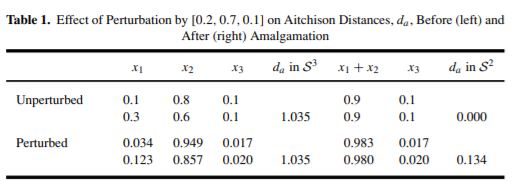
\includegraphics[scale=1.0]{ezogue_tab1.png}
%    \caption{Table from Egozcue et al. demonstrating alterations of sample distances after aggregation}
%    \label{fig:ezogue_tab1}
%\end{figure}

\subsection{Isometric log-ratio transformation}
One approach to solve this amalgamation issue is the isometric log ratio ($ilr$) transformation \cite{egozcue2003}. In essence, $ilr$ transform is a projection of the composition from the Aichison space to an orthonormal basis that exists in the simplex. This is different than the often use $alr$ and $clr$ transformations, where the This allows for the usage of standard statistical techniques as the composition is "opened" as well as being geometrically coherent compared to other flavors of log-ratio transforms. Conveniently, Egozcue et al. also showed that we can define a viable orthonormal basis from a sequential binary partition (SBP - which is a tree) \cite{egozcue2003}. The transformed $ilr$ coordinates are the tree nodes, which represent "balances" between two sides of the node. 
\begin{figure}[!htb]
    \centering
    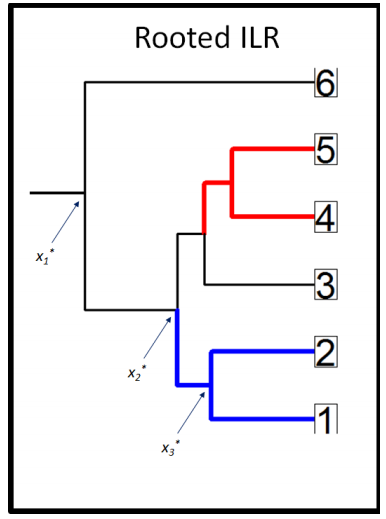
\includegraphics[scale = 0.5]{figures/phylogeny_demonstration.png}
    \caption{A sample SBP in tree form which is also the phylogenetic tree}
    \label{fig:figures/phylogeny_demonstration}
\end{figure}
Figure 2 is a toy example the ilr transformation on top of a phylogenetic tree. Each node $x_1^*, x_2^*, x_3^*$ represents the transformed ilr coordinates. The ilr transformation is defined as follows:
\begin{equation}
    x_i^* = \sqrt{\frac{l \cdot r}{r + l}} \log \left(\frac{g(\bm{x}_{j \in \bm{L}})}{g(\bm{x}_{j \in \bm{R}})}\right)
\end{equation}
where $\bm{x}$ is the compositional vector, $g()$ is the geometric mean, $\bm{L}$ is the set of size $l$ of all parts on the left side of the node, and $\bm R$ is the set of size $r$ of all parts on the left side of the node. Note that $\bm L$ and $\bm R$ are non-overlapping sets. For the example in Figure 2, we have: 
\[ x_2^* = \sqrt{\frac{2 \cdot 3}{2 + 3}} \log \left( \frac{(x_1x_2)^{1/2}}{(x_3x_4x_5)^{1/3}}\right) \]
The ilr coordinate can be interpreted as the overall relative contribution of variables in $\bm L$ to the composition of $\bm L \cup \bm R$ weighted by the sizes of $\bm L$ and $\bm R$. This concept of balances have gained recent attention by the microbiome field, targeting transformations and dimension reduction along the phylogenetic tree \cite{washburne2017a, silverman2017a}. Washburne et al. \cite{washburne2017a} argued that the $ilr$ uses ratios of geometric means, which is a more compositionally meaningful way to aggregate variables. Since the $ilr$ transformation naturally incorporates component comparison (as with all log-ratio techniques), it is a natural extension to perform competitive gene set enrichment (or taxonomic set enrichment - TSE), which tests the null hypothesis that genes in the gene set show more association with the outcome than those outside the gene set \cite{tian2005}. Roughly speaking, that null hypothesis can be rewritten as:
\begin{equation}
H_0 : \frac{\mathcal{A}(g \in G)_X}{\mathcal{A}(g \notin G)_X} = \frac{\mathcal{A}(g \in G)_Y}{\mathcal{A}(g \notin G)_Y}
\end{equation}
where $\mathcal{A}$ is a general aggregation function, $g$ represents genes, $G$ is a candidate gene set, $X$ and $Y$ are the case/control status. In other words, the competitive null hypothesis is that the relative enrichment of genes in gene set $G$ compared to those not in the gene set is the same across two conditions. As per the definition of the $ilr$ transformation, this is equivalent to testing the difference in $x^*_i$ in equation (2) between conditions $X$ and $Y$. As such, here we define a method that performs TSE using the $ilr$ transform as the test statistic, naturally incorporating both compositional data analysis as well as competitive set enrichment.     

\section{Methods}
\subsection{Taxonomic enrichment analysis using isometric log-ratio transformations (TEA-ILR)}
Here we propose a competitive taxonomic enrichment method based on an $ilr$ transformation of microbial compositions. Shortened as TRE-ILR.  
\vspace{3mm}

\noindent The TRE-ILR method takes in two matrices: 
\begin{itemize}
    \item $\bm X$: The $n \times p$ matrix of relative abundances of $p$ LT proportions in $n$ samples
    \item $\bm A$: The $m \times p$ matrix denoting the assignment of $p$ LT proportions into $m$ HT sets
\end{itemize}
TRE-ILR generates the following matrix: 
\begin{itemize}
    \item $\bm S$: The $n \times m$ matrix denoting the enrichment scores of $m$ HT sets by $n$ samples. 
\end{itemize}
With inputs $\bm{X}$ and $\bm{A}$, we compute $\bm{S}$ as follows:  
\begin{enumerate}
    \item Let $\bm{R}$ be a $n \times m$ matrix of competitive $ilr$ statistic for each HT set which is defined as follows:
    \begin{equation}
    R_{ij} = \sqrt{\frac{\sum_k A_{jk}(p - \sum_k A_{jk})}{p}} \log \left(\frac{g(\bm{x}_{ik} |A_{jk} \neq 0)}{g(\bm{x}_{ik} | A_{jk} = 0)}\right)
    \end{equation}
    \item To capture the distribution of the $ilr$ test statistic under the null hypothesis that the relative weights of LT proportions in the HT sets to the overall composition is no different than LT proportions not in the HT sets, the competitive $ilr$ statistic is computed for each HT set with permuting row labels of matrix $\bm{A}$, simulating random assignments of LTs into HT sets. Denote $\bm{A}_{perm}$ be the row-permuted version of $\bm{A}$ and $\bm{R}_{perm}$ be row-permuted version of $\bm{R}$
    \item We fit a gaussian distribution using the method of maximum likelihood for each column $\bm{R}_{perm}$. This stem from previous research treating the $ilr$ coordinates as normally distributed \cite{egozcue2005}.  
    \item Use the cumulative distribution (CDF) for the normal distribution to compute specific enrichment scores for HT sets. We formulate the target matrix $S$ as CDF scores for the normal distribution fitted on columns of $\bm{R}_{perm}$:
    \begin{equation}
        \bm{S}[,k] = F_{N(\hat{\mu}_{k},\hat{\sigma}_{k})}(\bm{R}_{perm}[,k])
    \end{equation}
\end{enumerate}

\subsection{TRE-ILR and standard isometric log-ratio transformations}
\noindent Let $\bm M$ be the $p-1 \times p$ sign matrix representing a sequential binary partition for $p$ ASVs across $p-1$ orders, with the first order being the first node from the root of the tree. For each sample $i$ we define $\mathcal{M}_i$ as the set of $\bm M$s such that 
\[ \mathcal{M}_i = \left\{\bm{M} | \bm{M}_{1j} = \begin{cases}
    1 \text{ if } A_{ij} = 1\\
    -1 \text{ if } A_{ij} = 0\\ 
\end{cases}
\right \}
\]
As such, $\mathcal{M}$ represents the set of SBPs such that the first order partition splits between the LT belonging to the HT set and those that don't. The $ilr$ coordinate of the first order partition is equal across all $\bm{M} \in \mathcal{M}$. In other words, we're interested in the coordinates for the projection of the composition $\bm{x}_{i}$ onto a very specific unit vector defined by the first order split as explained above.  
\[\bm{e}_i = \mathcal{C}[\exp(\underbrace{a, a, a,..., a, a, a}_{\sum_k A_{jk} \text{ elements}},\overbrace{b,b,b,...,b,b,b}^{p - \sum_k A_{jk} \text{ elements}}))] \]  
where $a = \sqrt{\frac{\sum_k A_{jk}}{p \cdot (p - \sum_k A_{jk})}}$ and $b = \sqrt{\frac{-(p - \sum_k A_{jk})}{p \cdot \sum_k A_{jk}}}$ with $\sum_k A_{jk}$ being the size of the HT set $k$ and $p - \sum_k A_{jk}$ being the number of LTs not in the HT set $k$. This unit vector can be part of various other orthonormal bases defined by the subtrees following the initial split. Since this vector is redefined for every HT set, the TRE-ILR $ilr$ coordinates can't be compared across sets without some sort of transformation.  
 
\subsection{Statistical properties of TRE-ILR}
Due to the equivalent of the TRE-ILR scores to the $ilr$ coordinates of the composition onto the unit vector $\bm{e}$ defined above, it enjoys the various statistical properties of the $ilr$ coordinate, specifically that it can be assumed to be normally distributed \cite{egozcue2003,egozcue2005}. As such, the raw TRE-ILR scores can be used for hypothesis testing for any specific HT set across two known case/control conditions. However, in order to use these scores together in a statistical model like a regression framework, we further transformed the scores as the CDF of the row-permuted distribution, which transforms the scores into a common scale. Furthermore, p-values associated to our null hypothesis can be obtained with a simple operation of $1 - S_{ij}$. Finally, it bounds the scores between 0 and 1, and is robust to large outliers.  

\section*{Simulation studies}



\newpage
\bibliography{tax_agg}{}
\bibliographystyle{plain}
\end{document}
\end{document}